\documentclass[12pt,a4paper]{report}

\usepackage[utf8]{inputenc}
\usepackage[T1]{fontenc}
\usepackage[french,english]{babel}
\usepackage[a4paper,margin=2.5cm]{geometry}
\usepackage[final]{graphicx}
\usepackage{float}
\usepackage{array}
\usepackage{booktabs}
\usepackage{tabularx}
\usepackage{longtable}
\usepackage{multirow}
\usepackage{listings}
\usepackage{xcolor}
\usepackage{titlesec}
\usepackage{fancyhdr}
\usepackage{caption}
\usepackage{enumitem}
\usepackage{hyperref}
\usepackage{setspace}
\usepackage{colortbl}
\usepackage{url}

\graphicspath{{./pfe_docs/}{./}{../pfe_docs/}}
\DeclareGraphicsExtensions{.pdf,.png,.jpg,.jpeg}
\setkeys{Gin}{draft=false}

\definecolor{moroccogreen}{HTML}{008060}
\definecolor{softgreen}{HTML}{E8F5F0}
\definecolor{lightgray}{HTML}{F5F7F8}
\definecolor{codebg}{HTML}{F7F9FA}
\definecolor{coderule}{HTML}{D9E2E7}

\hypersetup{
  colorlinks=true,
  linkcolor=moroccogreen,
  urlcolor=moroccogreen,
  citecolor=moroccogreen,
  pdftitle={MoroccoCheck -- Rapport PFE},
  pdfauthor={Abderrahmane BADDOU, Ahmed EL IDRISSI},
  pdfsubject={Projet de Fin d'Etudes},
  pdfkeywords={MoroccoCheck, tourisme, geolocalisation, Flutter, React, Node.js, PFE}
}

\titleformat{\chapter}[display]
  {\bfseries\Huge\color{moroccogreen}}
  {\filleft\MakeUppercase{\chaptertitlename}\ \thechapter}
  {1ex}
  {\titlerule\vspace{1ex}\filright}
  [\vspace{1ex}\titlerule]

\titleformat{\section}
  {\Large\bfseries\color{moroccogreen}}
  {\thesection}{1em}{}

\titleformat{\subsection}
  {\large\bfseries\color{moroccogreen}}
  {\thesubsection}{1em}{}
\titlespacing*{\chapter}{0pt}{-10pt}{18pt}
\titlespacing*{\section}{0pt}{14pt}{8pt}
\titlespacing*{\subsection}{0pt}{12pt}{6pt}

\pagestyle{fancy}
\fancyhf{}
\fancyhead[L]{MoroccoCheck}
\fancyhead[R]{Rapport PFE 2025--2026}
\fancyfoot[C]{\thepage}
\setlength{\headheight}{15pt}
\fancypagestyle{plain}{
  \fancyhf{}
  \fancyhead[L]{MoroccoCheck}
  \fancyhead[R]{Rapport PFE 2025--2026}
  \fancyfoot[C]{\thepage}
}

\renewcommand{\contentsname}{Table des mati\`eres}
\renewcommand{\listfigurename}{Liste des figures}
\renewcommand{\listtablename}{Liste des tableaux}
\renewcommand{\chaptername}{Chapitre}
\renewcommand{\bibname}{Bibliographie}

\setlist[itemize]{itemsep=0.4em}
\setlist[enumerate]{itemsep=0.4em}
\setstretch{1.15}
\setcounter{tocdepth}{2}
\setcounter{secnumdepth}{3}
\captionsetup{font=small,labelfont=bf}
\urlstyle{same}

\lstdefinestyle{moroccostyle}{
  backgroundcolor=\color{codebg},
  frame=single,
  rulecolor=\color{coderule},
  basicstyle=\ttfamily\small,
  keywordstyle=\color{moroccogreen}\bfseries,
  commentstyle=\color{gray},
  stringstyle=\color{orange!60!black},
  breaklines=true,
  showstringspaces=false,
  columns=fullflexible
}
\lstdefinelanguage{JavaScript}{
  keywords={const,let,var,function,return,if,else,async,await,try,catch,throw,import,from,export,default,class,extends,new,true,false,null},
  keywordstyle=\color{moroccogreen}\bfseries,
  ndkeywords={this},
  ndkeywordstyle=\color{moroccogreen}\bfseries,
  sensitive=true,
  comment=[l]{//},
  morecomment=[s]{/*}{*/},
  commentstyle=\color{gray},
  morestring=[b]',
  morestring=[b]",
  stringstyle=\color{orange!60!black}
}
\lstdefinelanguage{javascript}{
  keywords={const,let,var,function,return,if,else,async,await,try,catch,throw,import,from,export,default,class,extends,new,true,false,null},
  keywordstyle=\color{moroccogreen}\bfseries,
  ndkeywords={this},
  ndkeywordstyle=\color{moroccogreen}\bfseries,
  sensitive=true,
  comment=[l]{//},
  morecomment=[s]{/*}{*/},
  commentstyle=\color{gray},
  morestring=[b]',
  morestring=[b]",
  stringstyle=\color{orange!60!black}
}
\lstset{style=moroccostyle}

\newcolumntype{Y}{>{\raggedright\arraybackslash}X}

\begin{document}
\selectlanguage{french}

\begin{titlepage}
  \centering
  \vspace*{1cm}

  \noindent
  \begin{minipage}{0.48\textwidth}
    \raggedright
    
\includegraphics[width=0.38\textwidth]{logo_ESTA.jpeg}
  \end{minipage}
  \begin{minipage}{0.48\textwidth}
    \raggedleft
    
\includegraphics[width=0.22\textwidth]{00_logo_application_moroccocheck.png}
  \end{minipage}\\[0.8cm]

  {\Large \textbf{Universit\'e Ibn Zohr}}\\[0.2cm]
  {\large \'Ecole Sup\'erieure de Technologie d'Agadir (ESTA)}\\[0.2cm]
  {\large D\'epartement Informatique}\\[1cm]

  {\Huge\bfseries PROJET DE FIN D'\'ETUDES\\[0.25cm]}
  \textcolor{moroccogreen}{\rule{0.85\textwidth}{1.5pt}}\\[0.6cm]

  {\Large Pour l'obtention du dipl\^ome\\[0.2cm]}
  {\Large \textbf{DUT Conception et D\'eveloppement des Logiciels}}\\[0.9cm]

  {\LARGE\bfseries MoroccoCheck}\\[0.2cm]
  {\Large Plateforme touristique communautaire v\'erifi\'ee par g\'eolocalisation}\\[1cm]

  \renewcommand{\arraystretch}{1.35}
  \rowcolors{2}{lightgray}{white}
  \begin{tabularx}{0.95\textwidth}{>{\bfseries\color{moroccogreen}}p{4.2cm}Y}
    \toprule
    \'Etudiants & Abderrahmane BADDOU et Ahmed EL IDRISSI \\
    Fili\`ere & DUT Conception et D\'eveloppement des Logiciels \\
    \'Etablissement & \'Ecole Sup\'erieure de Technologie d'Agadir (ESTA) --- Universit\'e Ibn Zohr \\
    Encadrante & Pr. Aicha BAKKI \\
    Jury & Pr. Abderrahim SABOUR et Pr. Aicha BAKKI \\
    Soutenance & 30 mars 2026 \\
    Ann\'ee universitaire & 2025--2026 \\
    \bottomrule
  \end{tabularx}

  \vfill
  {\large Agadir, mars 2026}
\end{titlepage}

\pagenumbering{Roman}

\chapter*{D\'edicace}
\addcontentsline{toc}{chapter}{D\'edicace}
Nous d\'edica\c{c}ons ce travail \`a nos parents, pour leurs sacrifices, leur affection et leur soutien constant tout au long de notre parcours. Nous le d\'edica\c{c}ons \'egalement \`a nos familles, \`a nos proches et \`a toutes les personnes qui nous ont encourag\'es \`a pers\'ev\'erer. Enfin, nous d\'edions ce projet \`a toute personne qui voit dans la technologie un moyen concret de cr\'eer des solutions utiles, fiables et proches des besoins r\'eels des utilisateurs.

\clearpage
\chapter*{Remerciements}
\addcontentsline{toc}{chapter}{Remerciements}
Avant toute chose, nous rendons gr\^ace \`a Allah, Le Tout-Puissant, de nous avoir accord\'e la sant\'e, la patience, la volont\'e et la pers\'ev\'erance n\'ecessaires pour mener \`a bien ce projet de fin d'\'etudes.

Nous adressons nos plus profonds remerciements \`a nos parents et \`a nos familles pour leur soutien moral, leurs sacrifices, leurs encouragements permanents et la confiance qu'ils nous ont accord\'ee durant toutes nos ann\'ees d'\'etudes.

Nous exprimons notre sinc\`ere gratitude \`a notre encadrante p\'edagogique, Pr. Aicha BAKKI, pour la qualit\'e de son accompagnement, ses conseils, sa disponibilit\'e et la rigueur acad\'emique qu'elle nous a transmise tout au long de ce travail.

Nos remerciements vont \'egalement aux membres du jury, Pr. Abderrahim SABOUR et Pr. Aicha BAKKI, pour l'honneur qu'ils nous font en \'evaluant ce travail. Nous remercions aussi l'\'Ecole Sup\'erieure de Technologie d'Agadir, l'Universit\'e Ibn Zohr et l'ensemble des enseignants du D\'epartement Informatique pour la formation re\c{c}ue et l'encadrement assur\'e durant notre cursus.

\clearpage
\chapter*{R\'esum\'e}
\addcontentsline{toc}{chapter}{R\'esum\'e}
Le secteur touristique repose de plus en plus sur des informations num\'eriques diffus\'ees sur le web et sur mobile. Toutefois, ces informations sont souvent dispers\'ees, h\'et\'erog\`enes et parfois insuffisamment v\'erifi\'ees, ce qui limite leur fiabilit\'e pour les visiteurs. Dans ce contexte, MoroccoCheck a \'et\'e con\c{c}u comme une plateforme touristique communautaire focalis\'ee sur la consultation de lieux, la v\'erification terrain par g\'eolocalisation et la mod\'eration des contenus.

La solution d\'evelopp\'ee repose sur une architecture fullstack compos\'ee de trois sous-syst\`emes : une API REST Node.js / Express connect\'ee \`a une base MySQL, une application Flutter destin\'ee aux touristes, contributeurs et professionnels, et une interface React d\'edi\'ee \`a l'administration. Le syst\`eme permet notamment la gestion des comptes, la consultation des sites, la publication d'avis, la r\'ealisation de check-ins GPS, l'attribution de badges, la gestion professionnelle des \'etablissements et la mod\'eration centralis\'ee.

Sur le plan technique, le projet mobilise plusieurs technologies modernes, notamment Express, MySQL, Flutter, Provider, GoRouter, React, Firebase et Sentry. Les tests backend disponibles, l'organisation modulaire du code et les validations effectu\'ees montrent qu'une base fonctionnelle solide a \'et\'e mise en place. Le projet r\'epond ainsi \`a un besoin r\'eel de fiabilisation communautaire de l'information touristique, tout en offrant des perspectives d'\'evolution vers une plateforme plus large, plus analytique et plus riche en automatisation.

\noindent\textbf{Mots-cl\'es :} tourisme num\'erique, g\'eolocalisation, API REST, Flutter, mod\'eration, MySQL, application communautaire.

\clearpage
\chapter*{Abstract}
\addcontentsline{toc}{chapter}{Abstract}
\selectlanguage{english}
The tourism sector increasingly depends on digital information distributed through web and mobile platforms. However, such information is often scattered, heterogeneous and not always sufficiently verified, which reduces its reliability for visitors. In this context, MoroccoCheck was designed as a community-driven tourism platform focused on place discovery, on-site verification through geolocation and content moderation.

The implemented solution relies on a fullstack architecture composed of three main subsystems: a Node.js / Express REST API connected to a MySQL database, a Flutter application intended for tourists, contributors and professionals, and a React-based administration interface. The platform supports user account management, site browsing, review publication, GPS-based check-ins, badge attribution, professional venue management and centralized moderation workflows.

From a technical perspective, the project uses several modern technologies including Express, MySQL, Flutter, Provider, GoRouter, React, Firebase and Sentry. The available backend tests, the modular code organization and the validation steps carried out during the analysis indicate that a solid functional foundation has been established. The project therefore addresses a real need for community-based verification of tourism information while opening realistic perspectives for future extensions, richer analytics and more advanced automation capabilities.

\noindent\textbf{Keywords:} digital tourism, geolocation, REST API, Flutter, moderation, MySQL, community platform.
\selectlanguage{french}

\clearpage
\chapter*{Liste des abr\'eviations}
\addcontentsline{toc}{chapter}{Liste des abr\'eviations}
\begin{longtable}{p{3cm}p{11cm}}
\toprule
\textbf{Sigle} & \textbf{Signification} \\
\midrule
API & Application Programming Interface \\
REST & Representational State Transfer \\
JWT & JSON Web Token \\
GPS & Global Positioning System \\
UI & User Interface \\
UX & User Experience \\
SQL & Structured Query Language \\
CRUD & Create, Read, Update, Delete \\
CI & Continuous Integration \\
SPA & Single Page Application \\
KPI & Key Performance Indicator \\
PFE & Projet de Fin d'\'Etudes \\
ESTA & \'Ecole Sup\'erieure de Technologie d'Agadir \\
MCD & Mod\`ele Conceptuel de Donn\'ees \\
MLD & Mod\`ele Logique de Donn\'ees \\
MVC & Mod\`ele--Vue--Contr\^oleur \\
DTO & Data Transfer Object \\
HTTP & HyperText Transfer Protocol \\
CORS & Cross-Origin Resource Sharing \\
CORP & Cross-Origin-Resource-Policy \\
SDK & Software Development Kit \\
\bottomrule
\end{longtable}

\clearpage
\tableofcontents
\clearpage
\listoffigures
\clearpage
\listoftables

\clearpage
\pagenumbering{arabic}

\chapter{Cadre G\'en\'eral}

\section{Introduction g\'en\'erale}
La transformation num\'erique a profond\'ement modifi\'e les usages li\'es au tourisme. Les visiteurs s'appuient largement sur les applications mobiles, les cartes interactives, les avis en ligne et les r\'eseaux sociaux pour pr\'eparer un d\'eplacement, d\'ecouvrir un lieu ou organiser une activit\'e. Cette d\'ependance aux outils num\'eriques rend la qualit\'e, l'actualit\'e et la fiabilit\'e de l'information particuli\`erement importantes.

Dans ce contexte, MoroccoCheck se positionne comme une solution orient\'ee v\'erification communautaire. Le projet ne se limite pas \`a l'affichage de fiches touristiques : il int\`egre des check-ins g\'eolocalis\'es, des avis, un syst\`eme de progression, un espace professionnel et une interface d'administration. Cette orientation r\'epond \`a un besoin concret : disposer d'une information touristique plus fiable, mieux mod\'er\'ee et plus proche du terrain.

\section{Pr\'esentation de l'\'etablissement d'accueil}
L'\'Ecole Sup\'erieure de Technologie d'Agadir (ESTA), relevant de l'Universit\'e Ibn Zohr, assure une formation professionnalisante dans plusieurs disciplines technologiques. Le D\'epartement Informatique, dans lequel s'inscrit ce projet, vise \`a former des techniciens sup\'erieurs capables de concevoir, d\'evelopper, tester et maintenir des syst\`emes logiciels complets.

Le projet de fin d'\'etudes constitue une \'etape charni\`ere de ce parcours. Il permet de mobiliser simultan\'ement les comp\'etences en algorithmique, programmation web, bases de donn\'ees, g\'enie logiciel, assurance qualit\'e et communication technique.

\section{Pr\'esentation du projet MoroccoCheck}
MoroccoCheck est une plateforme fullstack compos\'ee de trois sous-syst\`emes compl\'ementaires :
\begin{itemize}
  \item une API REST Node.js / Express connect\'ee \`a MySQL ;
  \item une application Flutter destin\'ee aux touristes, contributeurs et professionnels ;
  \item une interface web React / Vite r\'eserv\'ee \`a l'administration.
\end{itemize}

L'objectif central du projet est de centraliser la consultation des sites touristiques, la contribution communautaire, la v\'erification sur place via GPS et la mod\'eration des contenus au sein d'un m\^eme \'ecosyst\`eme. La finalit\'e poursuivie n'est donc pas uniquement informative ; elle consiste \'egalement \`a renforcer la confiance accord\'ee aux contenus produits et consult\'es par les diff\'erents acteurs de la plateforme.

\section{Probl\'ematique}
Comment concevoir une plateforme touristique capable de centraliser des informations utiles sur les lieux \`a visiter tout en garantissant un meilleur niveau de confiance gr\^ace \`a la v\'erification g\'eolocalis\'ee, \`a la participation communautaire et \`a la mod\'eration des contenus ?

\section{Objectifs du projet}
\begin{itemize}
  \item Concevoir et d\'evelopper une plateforme fullstack d\'edi\'ee \`a la consultation et \`a la valorisation de lieux touristiques.
  \item Mettre en place une API REST s\'ecuris\'ee pour g\'erer utilisateurs, sites, avis, check-ins, badges et mod\'eration.
  \item Impl\'ementer une application Flutter ergonomique permettant la consultation mobile, les check-ins GPS et la gestion du profil.
  \item Fournir un espace professionnel pour la revendication et la gestion d'\'etablissements.
  \item Proposer un back-office d'administration permettant la mod\'eration des sites, des avis et des utilisateurs.
  \item Poser une base \'evolutive permettant l'ajout de nouvelles villes, d'analyses plus fines et de m\'ecanismes communautaires suppl\'ementaires.
\end{itemize}

\section{Acteurs et modules fonctionnels}
Les acteurs cibles identifi\'es dans le projet sont les visiteurs, les touristes authentifi\'es, les contributeurs, les professionnels et les administrateurs. Chaque profil dispose de parcours et de responsabilit\'es sp\'ecifiques.

\begin{table}[H]
\centering
\caption{Modules fonctionnels principaux de MoroccoCheck}
\begin{tabularx}{\textwidth}{p{4cm}Y}
\toprule
\textbf{Module} & \textbf{R\^ole dans le syst\`eme} \\
\midrule
Authentification et sessions & Inscription, connexion, gestion des tokens, renouvellement et d\'econnexion. \\
Catalogue touristique & Liste des sites, recherche, filtres, tri, fiche d\'etaill\'ee et consultation cartographique. \\
Check-in g\'eolocalis\'e & Validation de la pr\'esence sur site avec r\`egles de distance, pr\'ecision et preuves. \\
Avis et contributions & Publication d'avis, ajout de photos, interactions communautaires et r\'eponses propri\'etaires. \\
Gamification & Points, niveaux, badges, statistiques et classement. \\
Espace professionnel & Revendication d'un site, gestion des \'etablissements et suivi des statuts. \\
Administration & Mod\'eration des sites et avis, gestion des utilisateurs et des demandes contributor. \\
\bottomrule
\end{tabularx}
\end{table}

\section{Stack technique synth\'etique}
\begin{table}[H]
\centering
\caption{Principales technologies mobilis\'ees}
\begin{tabularx}{\textwidth}{p{4cm}p{3cm}Y}
\toprule
\textbf{Technologie} & \textbf{Version} & \textbf{Utilisation} \\
\midrule
Node.js / Express & 20.19.5 / 5.2.1 & Exposition de l'API REST et ex\'ecution de la logique serveur. \\
MySQL / mysql2 & 8.x / 3.16.2 & Persistance des donn\'ees m\'etier et connectivit\'e SQL. \\
Flutter / Dart & 3.38.7 / 3.10.7 & D\'eveloppement de l'application mobile et web. \\
Provider / GoRouter / Dio & 6.1.2 / 14.2.7 / 5.4.2 & Gestion d'\'etat, routage et appels HTTP dans Flutter. \\
React / Vite & 18.3.1 / 5.4.11 & Interface web d'administration et serveur de d\'eveloppement. \\
Firebase / Sentry & 12.11.0 / 10.46.0--9.16.0 & Authentification Google et supervision. \\
\bottomrule
\end{tabularx}
\end{table}

\section{Planification du projet}
La p\'eriode de r\'ealisation d\'eduite des documents du projet s'\'etend de d\'ecembre 2025 \`a mars 2026. La planification peut \^etre r\'esum\'ee comme suit.

\begin{table}[H]
\centering
\caption{Planning synth\'etique du projet}
\begin{tabularx}{\textwidth}{p{3cm}p{3cm}Y}
\toprule
\textbf{P\'eriode} & \textbf{Phase} & \textbf{Travaux r\'ealis\'es} \\
\midrule
D\'ecembre 2025 & Cadrage & Cahier des charges, d\'efinition du besoin, identification des acteurs et des objectifs. \\
Janvier 2026 & Conception & Mod\'elisation de la base de donn\'ees, structuration de l'architecture et des services. \\
F\'evrier 2026 & D\'eveloppement & Impl\'ementation du backend REST, de l'application Flutter et de l'admin React. \\
Mars 2026 & Stabilisation & Tests, corrections, documentation, captures d'\'ecran et pr\'eparation de la soutenance. \\
\bottomrule
\end{tabularx}
\end{table}

\section{Conclusion du chapitre}
Ce premier chapitre a permis de situer le projet dans son cadre institutionnel et fonctionnel. MoroccoCheck r\'epond \`a un besoin concret de fiabilisation de l'information touristique par une approche communautaire et g\'eolocalis\'ee. Le chapitre suivant pr\'esente l'analyse de l'existant, les besoins et la sp\'ecification de la solution.

\chapter{Analyse et Sp\'ecification}

\section{\'Etude de l'existant}
\subsection{Solutions existantes}
Avant de d\'evelopper MoroccoCheck, il a \'et\'e utile d'analyser plusieurs plateformes connues du domaine touristique.

\begin{table}[H]
\centering
\caption{Comparaison de quelques solutions existantes}
\begin{tabularx}{\textwidth}{p{2.2cm}p{3.2cm}Y p{2.7cm}}
\toprule
\textbf{Solution} & \textbf{Fonctionnalit\'es cl\'es} & \textbf{Limites vis-\`a-vis de MoroccoCheck} & \textbf{Fiabilit\'e par preuve de pr\'esence} \\
\midrule
TripAdvisor & Avis, notes, photos, classement de lieux, fiches d'\'etablissements. & Ne met pas la v\'erification GPS terrain au centre du fonctionnement. & Faible : les contributions ne sont pas conditionn\'ees \`a une pr\'esence physiquement contr\^ol\'ee. \\
Google Maps & Cartographie, itin\'eraires, fiches de lieux, avis et photos. & Orientation tr\`es large, sans logique communautaire locale de badges et de mod\'eration m\'etier d\'edi\'ee. & Faible : le flux principal n'int\`egre pas une preuve de pr\'esence GPS valid\'ee comme pivot de confiance. \\
Booking.com & R\'eservation, avis v\'erifi\'es, filtres avanc\'es. & Focalisation sur l'h\'ebergement et la r\'eservation, moins sur la validation communautaire de lieux vari\'es. & Moyenne : la fiabilit\'e repose surtout sur la transaction, non sur une validation terrain g\'eolocalis\'ee. \\
Yelp & Avis, notes, recherche locale, photos. & Faible int\'egration des processus de v\'erification terrain et de gestion professionnelle locale. & Faible : absence de preuve de pr\'esence instrument\'ee dans le parcours standard. \\
Culture Trip & Guides, recommandations, contenus \'editoriaux. & Orientation davantage \'editoriale que communautaire et transactionnelle. & Tr\`es faible : contenu orient\'e d\'ecouverte, sans contr\^ole de pr\'esence utilisateur sur le terrain. \\
\bottomrule
\end{tabularx}
\end{table}

\subsection{Critique de l'existant}
Les solutions existantes couvrent efficacement la recherche d'un lieu, la consultation d'avis ou la navigation. Toutefois, elles ne r\'epondent pas int\'egralement au positionnement observ\'e dans MoroccoCheck. Le projet met en avant une logique de v\'erification sur place avec contraintes GPS, rayon de validation variable, pr\'ecision minimale, gestion des photos de preuve et synchronisation hors ligne.

Par ailleurs, MoroccoCheck ne vise pas seulement la consultation d'informations, mais la constitution d'une communaut\'e locale et mod\'er\'ee autour du tourisme marocain. Le d\'eveloppement d'une solution sp\'ecifique est donc justifi\'e par le besoin d'unifier v\'erification terrain, participation communautaire, mod\'eration et pilotage m\'etier.

Le crit\`ere diff\'erenciateur majeur de la solution r\'eside donc dans la fiabilisation des donn\'ees par preuve de pr\'esence. MoroccoCheck rattache la contribution \`a un m\'ecanisme de check-in g\'eolocalis\'e qui tient compte de la distance au site, de la pr\'ecision GPS et de la d\'etection de positions simul\'ees. Cette orientation donne une coh\'erence forte \`a la probl\'ematique du projet et justifie la valeur ajout\'ee de la plateforme par rapport aux solutions g\'en\'eralistes du march\'e.

\section{Sp\'ecification des besoins}
\subsection{Besoins fonctionnels}
\begin{itemize}
  \item Le syst\`eme doit permettre \`a un visiteur de cr\'eer un compte via email et mot de passe.
  \item Le syst\`eme doit permettre \`a un utilisateur de se connecter via email / mot de passe et, lorsque disponible, via Google Sign-In.
  \item Le syst\`eme doit permettre la consultation, la recherche, le tri et le filtrage des sites touristiques.
  \item Le syst\`eme doit permettre \`a un utilisateur autoris\'e de r\'ealiser un check-in GPS sur un site.
  \item Le syst\`eme doit permettre la publication, la modification et la suppression d'avis.
  \item Le syst\`eme doit proposer un espace professionnel de revendication et de gestion d'\'etablissements.
  \item Le syst\`eme doit offrir une interface d'administration permettant la mod\'eration des sites, avis, utilisateurs et demandes contributor.
\end{itemize}

\subsection{Besoins non fonctionnels}
\begin{itemize}
  \item Performance : temps de r\'eponse compatibles avec un usage mobile.
  \item S\'ecurit\'e : protection des ressources via JWT, sessions, r\^oles, hachage des mots de passe, Helmet et CORS.
  \item Fiabilit\'e des donn\'ees : v\'erification GPS, contr\^ole de pr\'ecision et d\'etection de positions simul\'ees.
  \item Maintenabilit\'e : architecture en couches et s\'eparation claire des responsabilit\'es.
  \item Compatibilit\'e : fonctionnement sur mobile, web et interfaces desktop support\'ees par Flutter, ainsi que sur navigateur moderne pour l'administration.
  \item Observabilit\'e : endpoints de sant\'e, logs et int\'egration Sentry.
\end{itemize}

\section{Mod\'elisation UML}
\subsection{Diagramme de cas d'utilisation}
Le diagramme de cas d'utilisation met en \'evidence les principaux acteurs : visiteur, touriste authentifi\'e, contributeur, professionnel, administrateur et syst\`eme externe Google / Firebase. Il traduit les grands usages de la plateforme : consulter la carte, parcourir les sites, publier des avis, r\'ealiser un check-in, g\'erer des \'etablissements ou mod\'erer des contenus.

\begin{figure}[H]
  \centering
  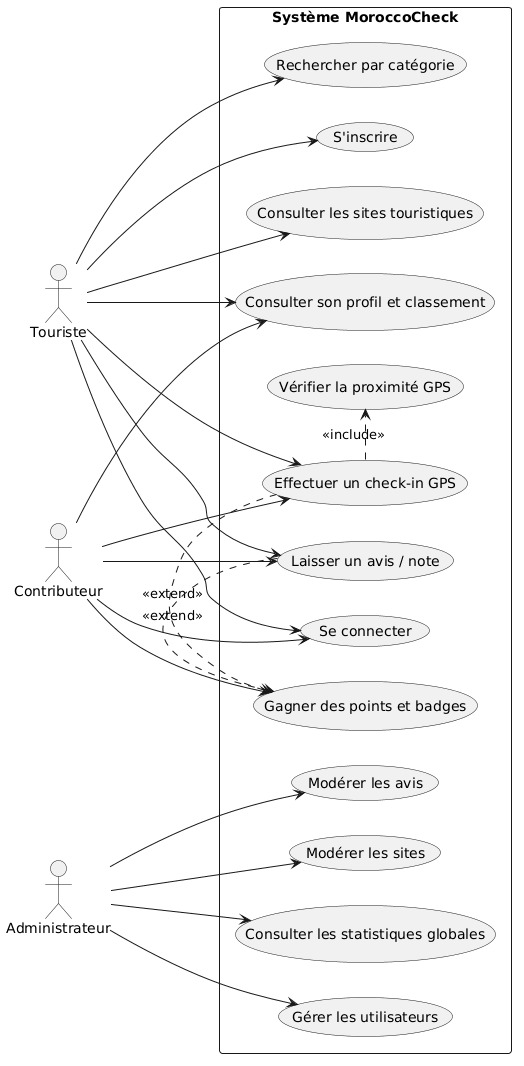
\includegraphics[width=0.62\textwidth,height=0.74\textheight,keepaspectratio]{05_diagramme_cas_utilisation_moroccocheck.jpeg}
  \caption{Diagramme de cas d'utilisation de MoroccoCheck}
\end{figure}

\subsection{Diagramme de classes}
Le diagramme de classes pr\'esente le noyau m\'etier du projet autour des entit\'es \texttt{User}, \texttt{TouristSite}, \texttt{Checkin}, \texttt{Review}, \texttt{Badge}, \texttt{Session} et \texttt{ContributorRequest}. Il montre aussi la relation entre les services m\'etier et les entit\'es manipul\'ees.

Pour enrichir sa lecture, les multiplicit\'es implicites les plus importantes peuvent \^etre rappel\'ees textuellement : un utilisateur peut poss\'eder plusieurs sessions, publier plusieurs avis et r\'ealiser plusieurs check-ins ; un site touristique peut recevoir plusieurs avis, photos et check-ins ; enfin, la relation entre utilisateurs et badges est de type plusieurs-\`a-plusieurs via \texttt{USER\_BADGES}. Les types de donn\'ees dominants observ\'es dans le sch\'ema SQL sont \texttt{INT}, \texttt{VARCHAR}, \texttt{TEXT}, \texttt{DECIMAL}, \texttt{DATETIME} et \texttt{ENUM}, ce qui confirme la coh\'erence du mod\`ele avec les besoins transactionnels et de mod\'eration.

\begin{figure}[H]
  \centering
  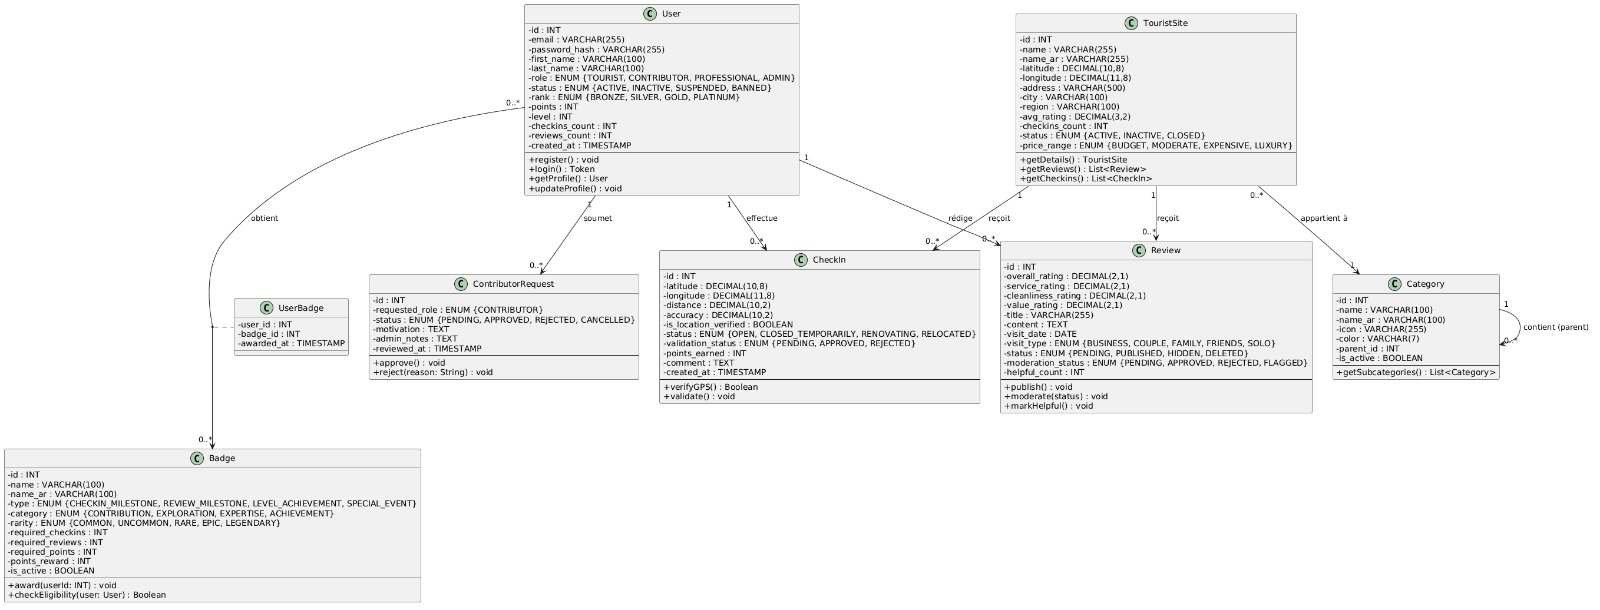
\includegraphics[width=0.95\textwidth]{06_diagramme_classes_moroccocheck.jpeg}
  \caption{Diagramme de classes de MoroccoCheck}
\end{figure}

\subsection{Diagramme d'activit\'e}
La gamification occupe une place importante dans l'engagement utilisateur. Le diagramme d'activit\'e ci-dessous illustre la logique de progression et d'attribution des badges \`a partir des check-ins, avis et actions r\'ealis\'ees dans l'application.

\begin{figure}[H]
  \centering
  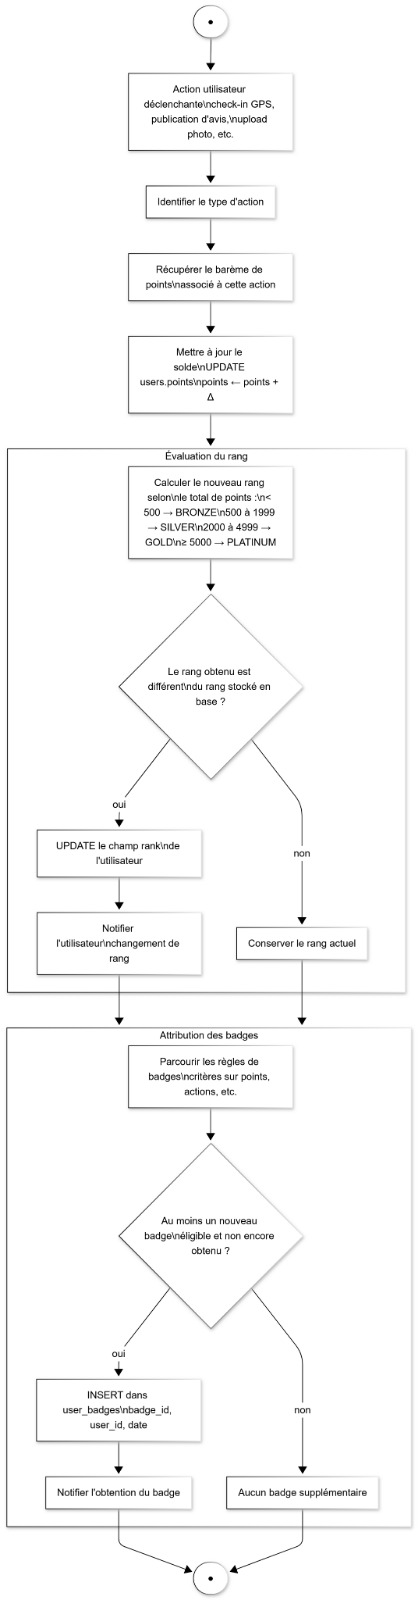
\includegraphics[width=0.42\textwidth,height=0.76\textheight,keepaspectratio]{07_diagramme_activite_gamification_badges.jpeg}
  \caption{Diagramme d'activit\'e de la gamification et des badges}
\end{figure}

\subsection{Diagramme de s\'equence}
Le sc\'enario de check-in GPS illustre l'un des parcours les plus sp\'ecifiques de la plateforme. Il met en jeu l'application Flutter, les services backend, les r\`egles de validation de distance et la mise \`a jour des statistiques.

\begin{figure}[H]
  \centering
  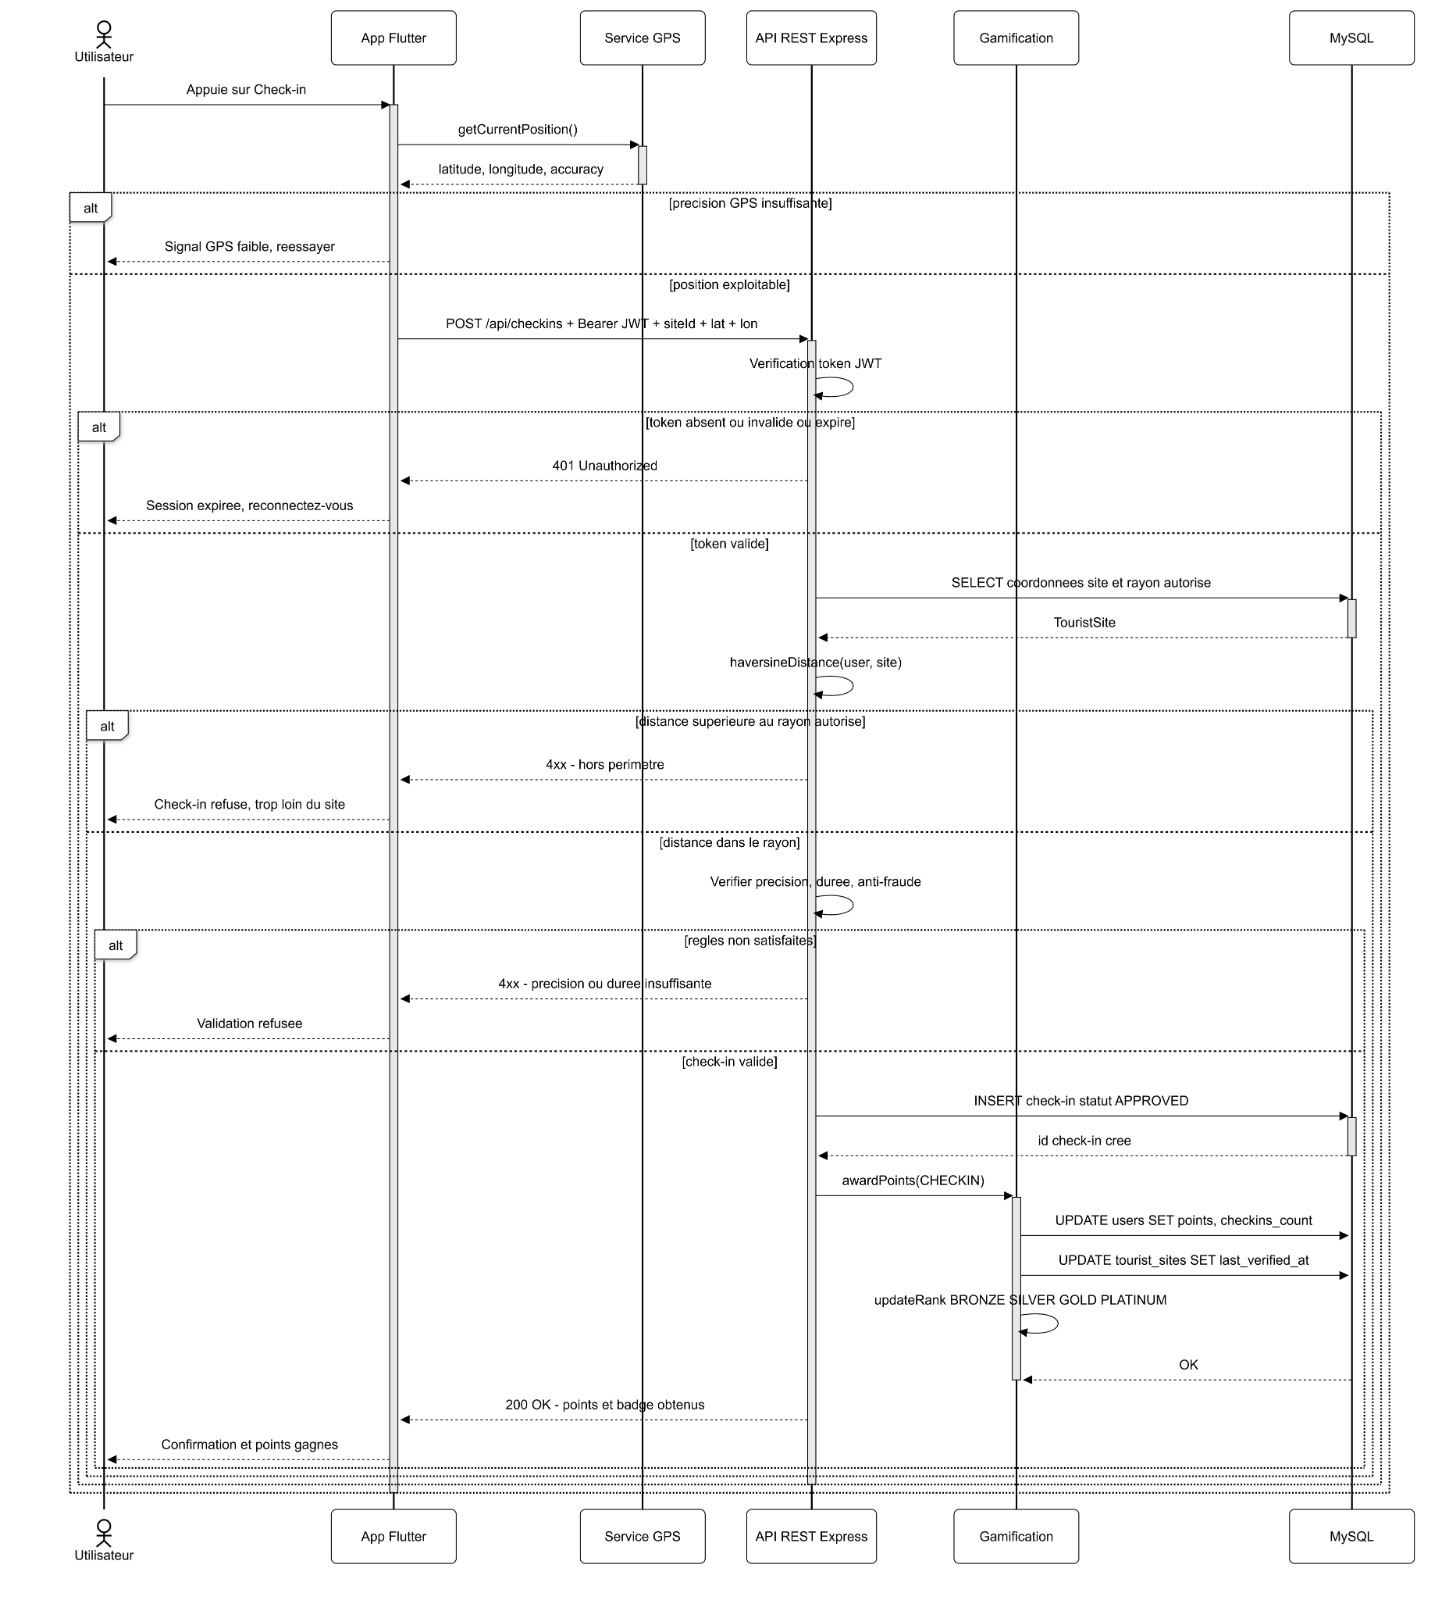
\includegraphics[width=0.92\textwidth]{08_diagramme_sequence_checkin_gps.jpeg}
  \caption{Diagramme de s\'equence du check-in g\'eolocalis\'e}
\end{figure}

Au-del\`a du flux nominal, ce sc\'enario comporte des branches d'erreur importantes pour l'analyse : refus du check-in si l'utilisateur est situ\'e hors du rayon autoris\'e, rejet lorsque la pr\'ecision GPS est insuffisante, et blocage lorsqu'une localisation simul\'ee est d\'etect\'ee. Ces cas sont coh\'erents avec les tests backend du projet et montrent que l'intelligence m\'etier ne repose pas uniquement sur l'interface, mais aussi sur des validations robustes c\^ot\'e serveur.

\section{Conclusion du chapitre}
L'analyse de l'existant et des besoins montre que MoroccoCheck d\'epasse le cadre d'une simple application de consultation touristique. Le projet articule un catalogue de lieux, une v\'erification terrain par g\'eolocalisation, des m\'ecanismes communautaires, un espace professionnel et une administration de mod\'eration. Le chapitre suivant pr\'esente l'\'etude technique retenue pour supporter ces exigences.

\chapter{\'Etude Technique}

\section{Architecture globale}
L'architecture retenue est une architecture client--serveur en trois sous-syst\`emes compl\'ementaires. Le backend \texttt{back-end/} constitue le noyau central. Il expose une API REST construite avec Express 5 et organis\'ee selon une s\'eparation \texttt{routes -> controllers -> services -> utils / middleware / config}. Le client Flutter \texttt{front-end/} s'appuie sur Provider pour la gestion d'\'etat, GoRouter pour la navigation et Dio pour les appels HTTP. Enfin, \texttt{admin-web/} fournit une interface web d'administration en React 18 et Vite, r\'eserv\'ee aux comptes \texttt{ADMIN}.

Cette organisation traduit un choix d'architecture pragmatique et lisible : elle s\'epare nettement les responsabilit\'es techniques, facilite la maintenance du syst\`eme et permet de faire \'evoluer ind\'ependamment les interfaces de consultation et de gouvernance, tout en conservant une couche m\'etier unifi\'ee c\^ot\'e serveur.

\begin{figure}[H]
  \centering
  \fcolorbox{moroccogreen}{softgreen}{
    \parbox{0.92\textwidth}{
      \centering
      \textbf{Utilisateurs mobile/web} \hspace{1cm} \textbf{Administrateur}\\[0.2cm]
      Application Flutter \hspace{2cm} Interface React Admin\\[0.4cm]
      \rule{0.8\textwidth}{0.4pt}\\[0.4cm]
      API REST Node.js / Express\\[0.2cm]
      Authentification, sites, check-ins, avis, badges, mod\'eration\\[0.4cm]
      \rule{0.8\textwidth}{0.4pt}\\[0.4cm]
      MySQL \hspace{0.8cm} Firebase/Google \hspace{0.8cm} Sentry \hspace{0.8cm} Redis optionnel
    }
  }
  \caption{Vue d'ensemble de l'architecture technique de MoroccoCheck}
\end{figure}

\section{Organisation du backend selon une logique MVC}
Le backend adopte une organisation modulaire proche du mod\`ele MVC, adapt\'ee aux API REST. Les routes d\'efinissent les points d'entr\'ee HTTP, les controllers adaptent les requ\^etes aux cas d'usage m\'etier, les services encapsulent la logique fonctionnelle et les acc\`es SQL, tandis que les utilitaires et middlewares prennent en charge la validation, la gestion des erreurs, les uploads et la s\'ecurit\'e.

\begin{lstlisting}[language=bash,caption={Arborescence simplifi\'ee du projet}]
App_Touriste/
|-- back-end/
|   |-- src/
|   |   |-- config/
|   |   |-- controllers/
|   |   |-- middleware/
|   |   |-- routes/
|   |   |-- services/
|   |   `-- utils/
|-- front-end/
|   `-- lib/
|       |-- core/
|       |-- features/
|       `-- shared/
`-- admin-web/
    `-- src/
\end{lstlisting}

\section{S\'ecurit\'e et fiabilit\'e}
La s\'ecurit\'e constitue une exigence structurante du projet. Plusieurs m\'ecanismes sont observables dans le code source :
\begin{itemize}
  \item authentification par JWT et conservation des sessions dans la base de donn\'ees ;
  \item v\'erification des r\^oles pour prot\'eger les routes sensibles ;
  \item hachage des mots de passe via \texttt{bcryptjs} ;
  \item validation des donn\'ees entrantes via Joi ;
  \item durcissement HTTP via Helmet ;
  \item configuration CORS et gestion des erreurs centralis\'ee ;
  \item r\`egles m\'etier sp\'ecifiques pour les check-ins GPS.
\end{itemize}

L'analyse du code source permet d'apporter des pr\'ecisions suppl\'ementaires sur la gestion des secrets et le stockage des jetons. C\^ot\'e backend, la signature des JWT d\'epend d'un secret charg\'e depuis les variables d'environnement (\texttt{JWT\_SECRET}) ainsi que d'une dur\'ee de vie configurable (\texttt{JWT\_EXPIRES\_IN}). C\^ot\'e application Flutter, les jetons d'acc\`es et de rafra\^\i chissement sont stock\'es via \texttt{FlutterSecureStorage}, avec activation des \texttt{encryptedSharedPreferences} sur Android. C\^ot\'e administration web, le jeton est actuellement persist\'e dans \texttt{localStorage} afin de simplifier le back-office ; dans une perspective de durcissement suppl\'ementaire, une \'evolution vers des cookies \texttt{HttpOnly} constituerait une am\'elioration pertinente.

\begin{lstlisting}[language=JavaScript,caption={Extrait illustratif de la cr\'eation d'une session}]
async function createSession(db, user, requestContext = {}) {
  const accessToken = generateToken(user);
  const refreshToken = randomBytes(32).toString('hex');

  await db.query(
    `INSERT INTO sessions (
      id, user_id, access_token, refresh_token, ip_address, expires_at
    ) VALUES (?, ?, ?, ?, ?, DATE_ADD(NOW(), INTERVAL ? DAY))`,
    [
      randomUUID(),
      user.id,
      accessToken,
      refreshToken,
      requestContext.ipAddress || '0.0.0.0',
      REFRESH_TOKEN_TTL_DAYS
    ]
  );
}
\end{lstlisting}

\section{Conception de la base de donn\'ees}
Le mod\`ele de donn\'ees est riche et centr\'e sur les entit\'es \texttt{USERS}, \texttt{TOURIST\_SITES}, \texttt{CHECKINS}, \texttt{REVIEWS}, \texttt{BADGES}, \texttt{USER\_BADGES}, \texttt{PHOTOS} et \texttt{SESSIONS}. Cette mod\'elisation prend en charge \`a la fois la consultation, la contribution, la mod\'eration et la tra\c{c}abilit\'e.

\begin{table}[H]
\centering
\caption{Tables principales de la base de donn\'ees}
\begin{tabularx}{\textwidth}{p{4cm}Y}
\toprule
\textbf{Table} & \textbf{R\^ole} \\
\midrule
USERS & Comptes, r\^oles, statuts, progression, informations de profil. \\
TOURIST\_SITES & Fiches des lieux touristiques, cat\'egories, coordonn\'ees et statuts de validation. \\
CHECKINS & Historique des validations terrain, position, pr\'ecision et notes de v\'erification. \\
REVIEWS & Avis, notes, contenus textuels, mod\'eration et r\'eponses propri\'etaires. \\
BADGES / USER\_BADGES & Gestion de la gamification et de la progression communautaire. \\
CONTRIBUTOR\_REQUESTS & Workflow de changement de r\^ole pour les touristes souhaitant devenir contributeurs. \\
PHOTOS & Fichiers m\'edias associ\'es aux sites, avis et preuves de check-in. \\
SESSIONS & Stockage des sessions actives, refresh tokens et m\'etadonn\'ees de connexion. \\
\bottomrule
\end{tabularx}
\end{table}

\begin{figure}[H]
  \centering
  \fcolorbox{moroccogreen}{lightgray}{
    \parbox{0.94\textwidth}{
      \centering
      \renewcommand{\arraystretch}{1.2}
      \begin{tabularx}{0.92\textwidth}{>{\bfseries}p{4cm}Y}
      USERS & 1,n SESSIONS ; 1,n CHECKINS ; 1,n REVIEWS ; 1,n CONTRIBUTOR\_REQUESTS ; n,n BADGES via USER\_BADGES \\
      TOURIST\_SITES & 1,n CHECKINS ; 1,n REVIEWS ; 1,n PHOTOS ; 0,1 propri\'etaire professionnel r\'ef\'erenc\'e dans USERS \\
      CHECKINS & n,1 USERS ; n,1 TOURIST\_SITES ; 0,n PHOTOS de preuve \\
      REVIEWS & n,1 USERS ; n,1 TOURIST\_SITES ; 0,n PHOTOS ; r\'eponse propri\'etaire optionnelle \\
      BADGES / USER\_BADGES & Catalogue des badges et table d'association pour l'attribution aux utilisateurs \\
      SESSIONS & n,1 USERS ; support du cycle login, refresh token et d\'econnexion \\
      \end{tabularx}
    }
  }
  \caption{Vue synth\'etique du mod\`ele logique de donn\'ees (MLD)}
\end{figure}

\begin{lstlisting}[language=SQL,caption={Extrait de DDL illustratif inspir\'e du sch\'ema du projet}]
CREATE TABLE users (
  id INT AUTO_INCREMENT PRIMARY KEY,
  email VARCHAR(255) NOT NULL UNIQUE,
  password_hash VARCHAR(255) NOT NULL,
  first_name VARCHAR(100) NOT NULL,
  last_name VARCHAR(100) NOT NULL,
  role ENUM('TOURIST','CONTRIBUTOR','PROFESSIONAL','ADMIN') NOT NULL,
  status ENUM('ACTIVE','INACTIVE','SUSPENDED') NOT NULL DEFAULT 'ACTIVE',
  points INT NOT NULL DEFAULT 0,
  level INT NOT NULL DEFAULT 1,
  rank VARCHAR(50) DEFAULT 'BRONZE'
);
\end{lstlisting}

\section{Clients Flutter et React Admin}
L'application Flutter constitue le client principal c\^ot\'e utilisateur. Elle g\`ere la navigation, la carte, le catalogue touristique, le profil, les check-ins et l'espace professionnel. L'interface React Admin se concentre sur les op\'erations de mod\'eration, de supervision et de gouvernance.

Ce choix hybride r\'epond \`a une justification technique et ergonomique nette. Flutter est adapt\'e au client principal car il facilite une exp\'erience mobile fluide, l'int\'egration de la g\'eolocalisation, l'affichage cartographique et les interactions de terrain \`a partir d'une base de code unifi\'ee. \`A l'inverse, l'administration requiert surtout des tableaux denses, des filtres, des formulaires et des tableaux de bord ; dans ce contexte, React offre une excellente r\'eactivit\'e pour le back-office, un d\'eploiement navigateur imm\'ediat et une maintenance rapide des vues de supervision.

La s\'eparation des clients pr\'esente plusieurs avantages :
\begin{itemize}
  \item sp\'ecialisation ergonomique selon le profil d'usage ;
  \item simplification des parcours m\'etier ;
  \item meilleure ma\^\i trise des droits d'acc\`es ;
  \item possibilit\'e de faire \'evoluer les interfaces ind\'ependamment.
\end{itemize}

\section{Conclusion du chapitre}
L'\'etude technique montre que MoroccoCheck repose sur une base logicielle coh\'erente et \'evolutive. L'architecture \`a trois sous-syst\`emes, la structuration modulaire du backend, la richesse du mod\`ele de donn\'ees et les m\'ecanismes de s\'ecurit\'e constituent des fondations solides pour la r\'ealisation pr\'esent\'ee dans le chapitre suivant.

\chapter{R\'ealisation}

\section{Environnement de d\'eveloppement}
Le projet a \'et\'e r\'ealis\'e dans un environnement moderne combinant Node.js, MySQL, Flutter, React, Firebase et Sentry. Les outils de d\'eveloppement observ\'es dans le d\'ep\^ot incluent notamment Git, GitHub Actions, Mocha, Chai, Supertest, Vitest et Flutter Test. Cet environnement t\'emoigne d'une volont\'e de couvrir l'ensemble du cycle de vie logiciel, depuis le d\'eveloppement jusqu'\`a la validation et \`a la supervision.

\section{Fonctionnalit\'es majeures impl\'ement\'ees}
L'impl\'ementation concr\`ete du projet couvre les fonctionnalit\'es essentielles suivantes :
\begin{itemize}
  \item gestion des sessions et authentification utilisateur ;
  \item catalogue touristique avec recherche, filtres et consultation cartographique ;
  \item check-ins g\'eolocalis\'es avec r\`egles de validation ;
  \item publication d'avis et gestion des contenus communautaires ;
  \item gamification avec points, badges et classement ;
  \item espace professionnel de gestion des \'etablissements ;
  \item interface de mod\'eration et de supervision pour l'administration.
\end{itemize}

\begin{lstlisting}[language=JavaScript,caption={Exemple d'endpoint de mod\'eration c\^ot\'e backend}]
router.use(adminRateLimit, authMiddleware, authorizeRoles('ADMIN'));

router.get('/sites/pending', asyncHandler(getPendingSites));
router.get('/reviews/pending', asyncHandler(getPendingReviews));
router.put('/reviews/:id/moderate', asyncHandler(moderateReviewHandler));
router.get('/stats', asyncHandler(getAdminStatsHandler));
\end{lstlisting}

\section{Interfaces de l'application}
Cette section pr\'esente les principales interfaces fonctionnelles du syst\`eme. Chaque capture a \'et\'e retenue pour illustrer un parcours significatif et mettre en \'evidence sa valeur fonctionnelle pour l'utilisateur final ou pour l'administrateur.

\subsection{Connexion utilisateur}
L'interface de connexion permet d'ouvrir une session via email et mot de passe, avec une possibilit\'e de connexion Google lorsque la configuration Firebase est compl\`ete.

\begin{figure}[H]
  \centering
  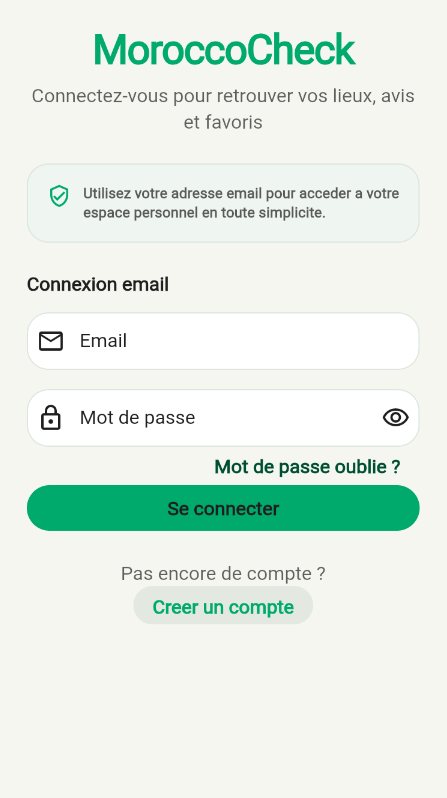
\includegraphics[width=0.34\textwidth]{01_ecran_connexion_utilisateur.png}
  \caption{Interface d'authentification donnant acc\`es aux parcours personnalis\'es et aux contributions communautaires.}
\end{figure}

\subsection{Espace professionnel : actions rapides}
Cet \'ecran pr\'esente le point d'entr\'ee de l'espace professionnel et met en avant les raccourcis m\'etier utiles pour revendiquer ou administrer un \'etablissement.

\begin{figure}[H]
  \centering
  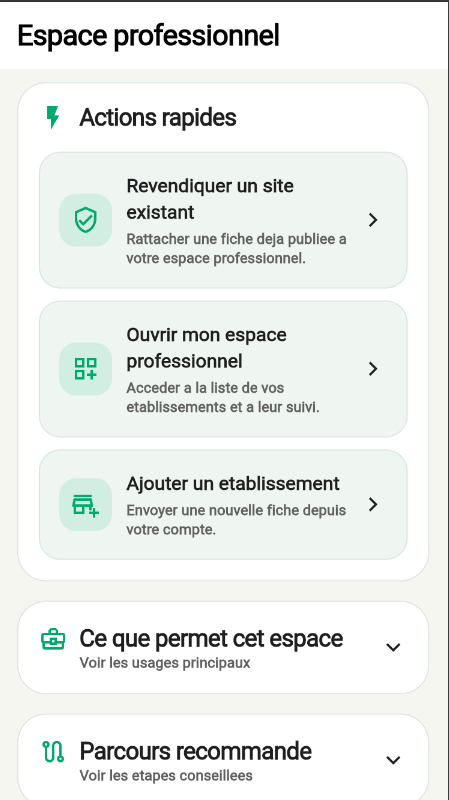
\includegraphics[width=0.34\textwidth]{02_ecran_espace_professionnel_actions_rapides.png}
  \caption{Point d'entr\'ee m\'etier regroupant les actions prioritaires du professionnel pour administrer sa pr\'esence sur la plateforme.}
\end{figure}

\subsection{Gestion des \'etablissements professionnels}
Cette vue permet au professionnel de suivre les lieux qu'il g\`ere, d'observer les indicateurs principaux et d'acc\'eder rapidement aux actions de pilotage.

\begin{figure}[H]
  \centering
  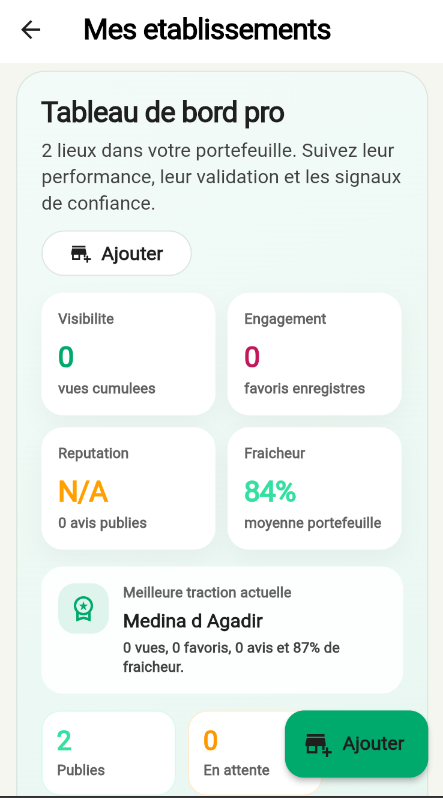
\includegraphics[width=0.34\textwidth]{03_ecran_mes_etablissements_professionnel.png}
  \caption{Vue de pilotage des \'etablissements g\'er\'es, utile pour le suivi op\'erationnel, les statuts et les indicateurs d'activit\'e.}
\end{figure}

\subsection{Liste des sites touristiques}
L'\'ecran de liste facilite l'exploration du catalogue par recherche textuelle, cat\'egorie, tri et pr\'evisualisation des cartes de lieux.

\begin{figure}[H]
  \centering
  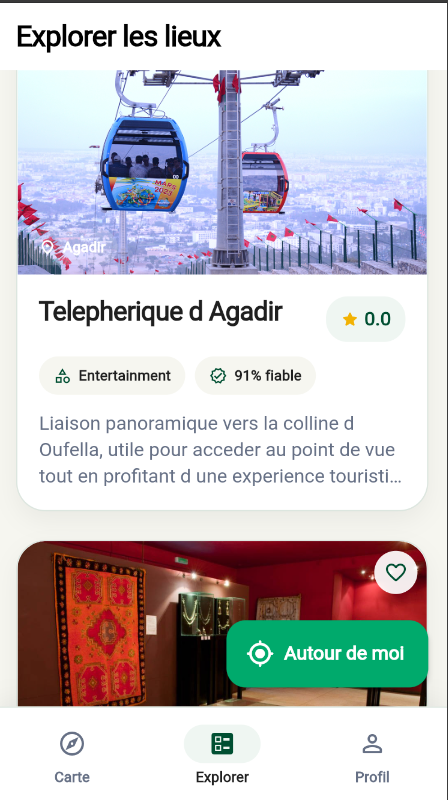
\includegraphics[width=0.34\textwidth]{04_ecran_liste_sites_touristiques.png}
  \caption{Catalogue mobile orient\'e d\'ecouverte, combinant recherche, tri et acc\`es rapide aux lieux touristiques r\'ef\'erenc\'es.}
\end{figure}

\subsection{Carte d'Agadir}
La carte constitue une interface centrale du projet. Elle visualise les lieux touristiques, les filtres de consultation et la logique de recentrage spatial.

\begin{figure}[H]
  \centering
  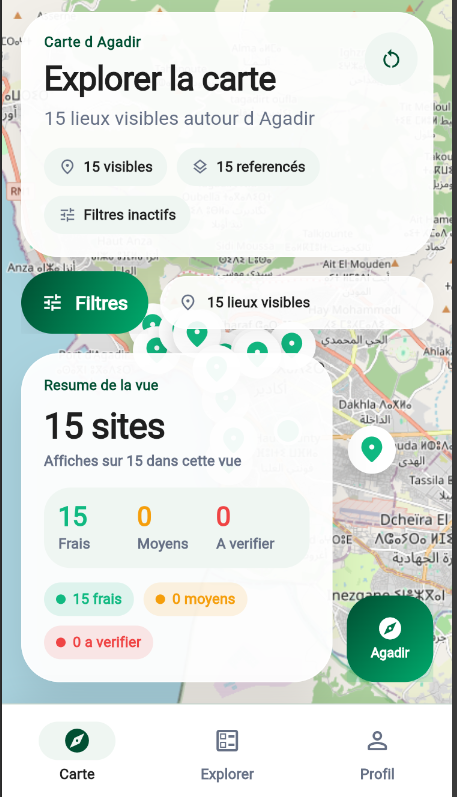
\includegraphics[width=0.34\textwidth]{05_ecran_carte_agadir.png}
  \caption{Visualisation cartographique des lieux filtr\'es, con\c{c}ue pour articuler exploration spatiale et aide \`a la d\'ecision sur le terrain.}
\end{figure}

\subsection{D\'etail d'un site}
La fiche de site rassemble les informations essentielles : identit\'e du lieu, contenus visuels, description, horaires, avis, contact et actions de contribution.

\begin{figure}[H]
  \centering
  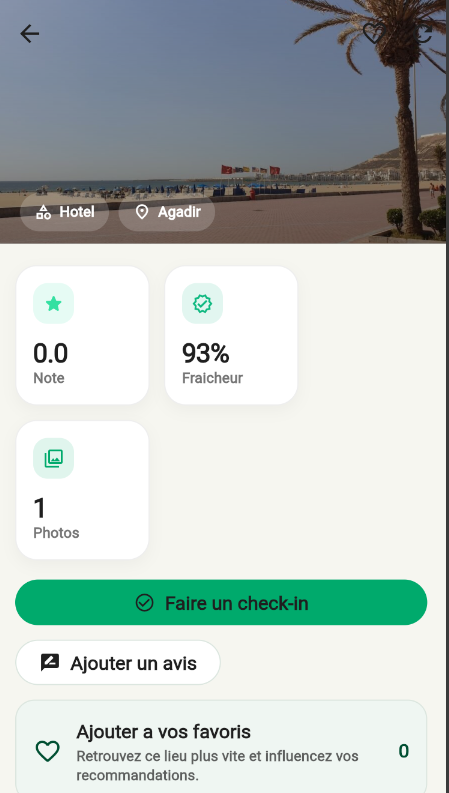
\includegraphics[width=0.34\textwidth]{06_ecran_detail_site_touristique.png}
  \caption{Fiche de r\'ef\'erence d'un lieu, consolidant contenu descriptif, informations de confiance et actions de contribution.}
\end{figure}

\subsection{Check-in g\'eolocalis\'e}
Le check-in illustre le caract\`ere sp\'ecifique du projet. L'interface guide l'utilisateur dans la validation de sa pr\'esence sur le terrain en tenant compte de la g\'eolocalisation et de la qualit\'e de la mesure.

\begin{figure}[H]
  \centering
  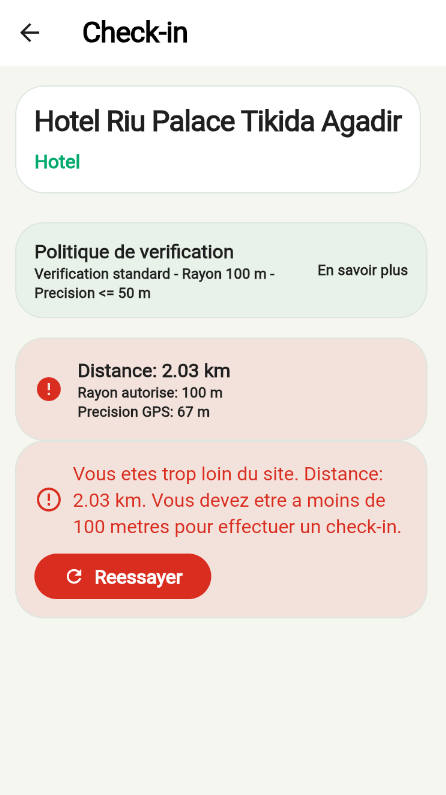
\includegraphics[width=0.34\textwidth]{07_ecran_checkin_geolocalise.png}
  \caption{Workflow de validation de pr\'esence sur site, au coeur de la promesse de fiabilisation port\'ee par MoroccoCheck.}
\end{figure}

\subsection{Connexion administrateur}
L'interface d'acc\`es administrateur permet l'authentification au back-office de gouvernance et de mod\'eration de la plateforme.

\begin{figure}[H]
  \centering
  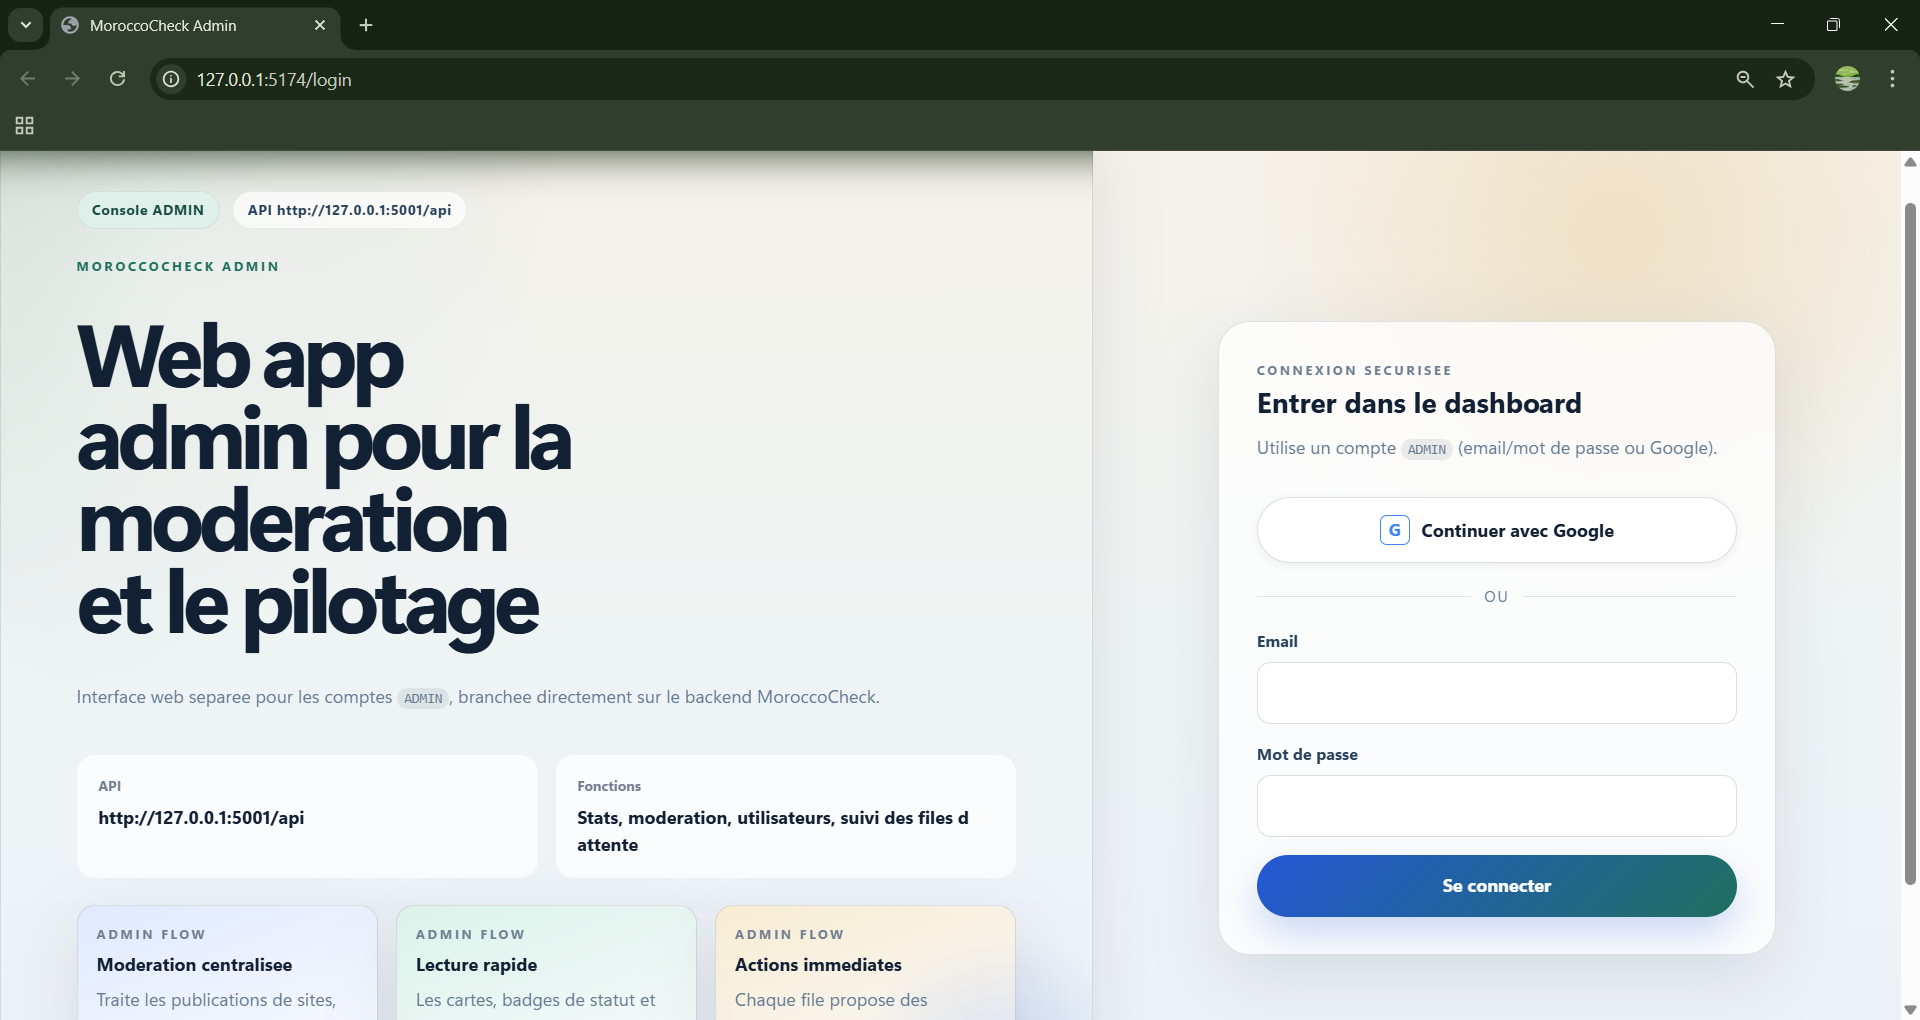
\includegraphics[width=0.90\textwidth]{08_ecran_connexion_admin.png}
  \caption{Point de contr\^ole s\'ecuris\'e donnant acc\`es aux fonctions de gouvernance et de mod\'eration du back-office.}
\end{figure}

\subsection{Tableau de bord administrateur}
Le tableau de bord administrateur centralise les statistiques de supervision, les files d'attente de traitement et les indicateurs de pilotage op\'erationnel.

\begin{figure}[H]
  \centering
  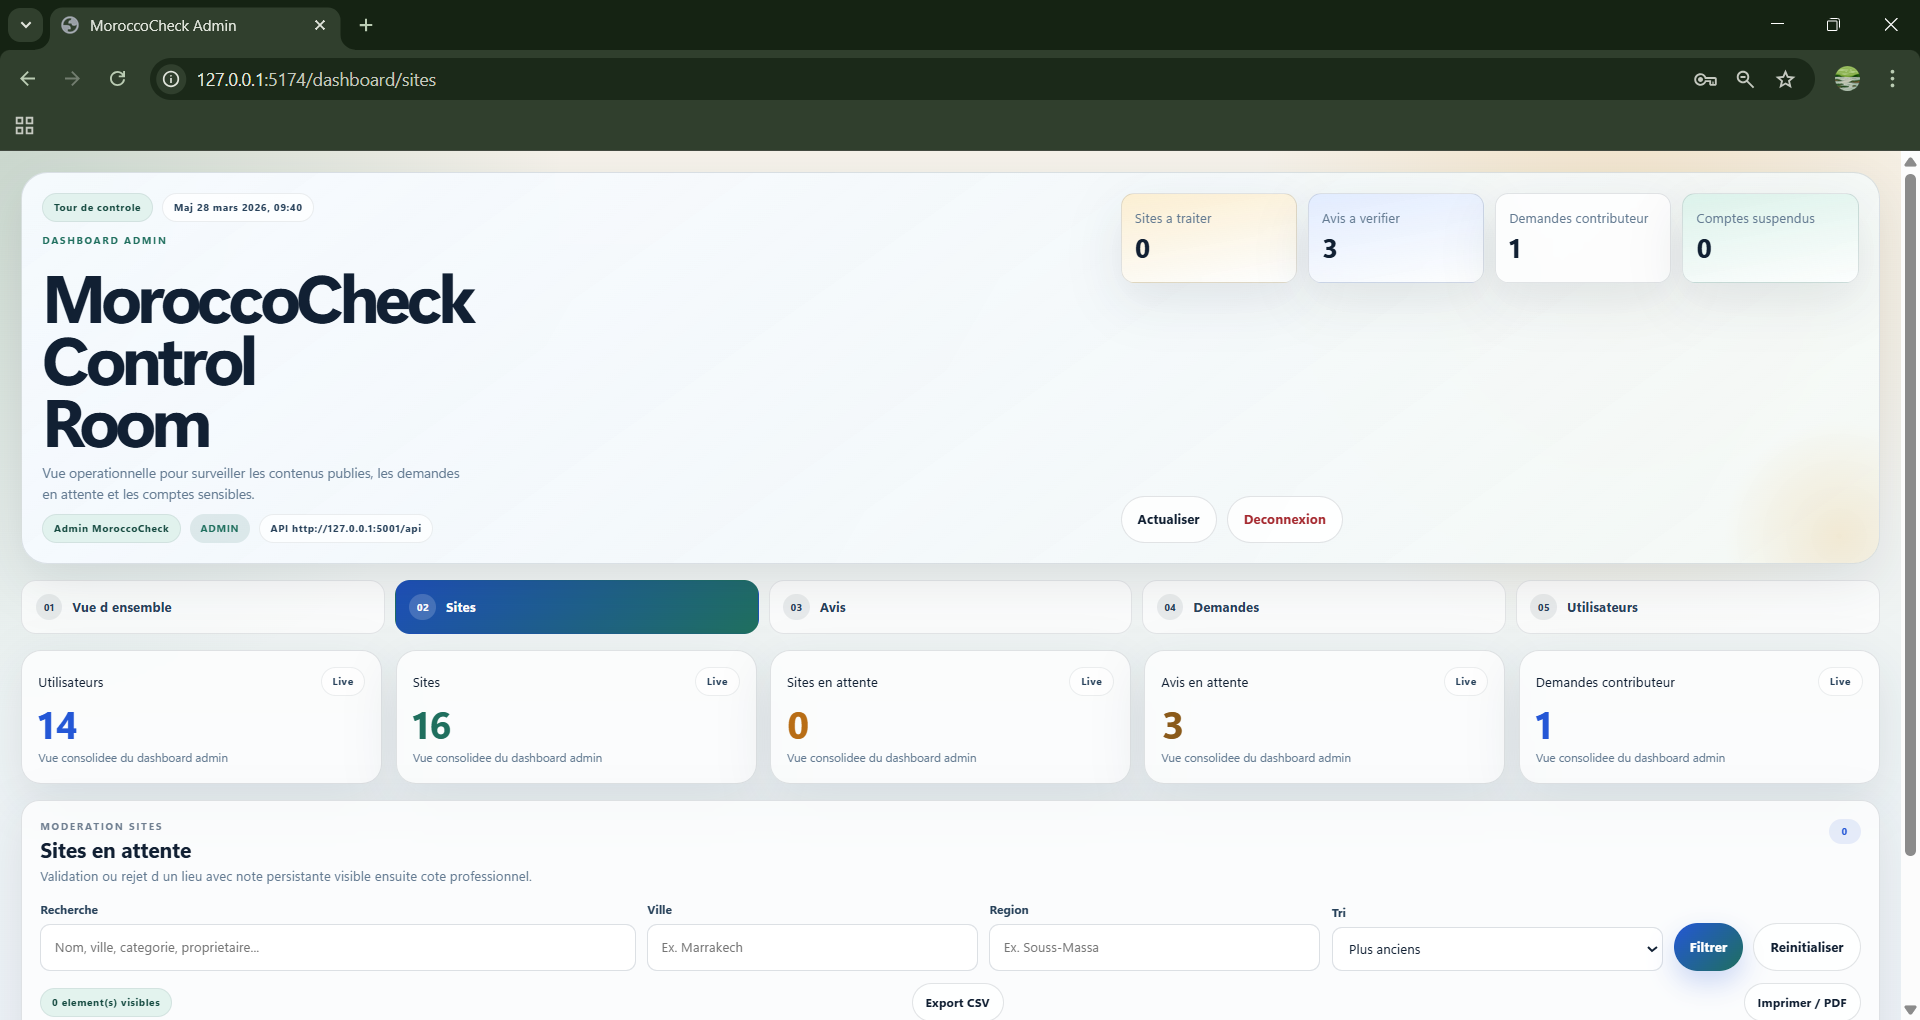
\includegraphics[width=0.90\textwidth]{09_ecran_tableau_bord_admin.png}
  \caption{Poste de supervision centralisant les files d'attente, les indicateurs et les d\'ecisions de mod\'eration.}
\end{figure}

\section{Tests et validation}
Le projet dispose de plusieurs niveaux de validation formelle :
\begin{itemize}
  \item des tests backend dans \texttt{back-end/tests/} avec Mocha, Chai et Supertest ;
  \item des tests d'interface admin avec Vitest ;
  \item des tests Flutter pr\'esents dans \texttt{front-end/test/}.
\end{itemize}

\begin{table}[H]
\centering
\caption{Synth\`ese des dispositifs de validation observables dans le d\'ep\^ot}
\begin{tabularx}{\textwidth}{p{4cm}p{3cm}Y}
\toprule
\textbf{Composant} & \textbf{\'El\'ements identifi\'es} & \textbf{Commentaire} \\
\midrule
Backend Node.js & 53 cas de test & Couverture significative de l'authentification, de la sant\'e applicative, des cat\'egories, des sites, des avis, des check-ins, des middlewares et du module d'administration. \\
Admin React & 3 tests unitaires & Validation cibl\'ee de la normalisation et de la r\'esolution de l'URL API, utile pour la robustesse du back-office. \\
Frontend Flutter & 5 tests widgets & Les tests portent sur le routage prot\'eg\'e, l'\'ecran de check-in, le d\'etail d'un site et le classement ; ils doivent \^etre maintenus \`a chaque \'evolution de l'interface et des libell\'es. \\
\bottomrule
\end{tabularx}
\end{table}

Cette pr\'esentation appelle une nuance importante : la pr\'esence de suites de test dans le d\'ep\^ot constitue un indicateur positif de qualit\'e, mais ne remplace pas une ex\'ecution consolid\'ee et horodat\'ee avant la soutenance. Dans le cas de Flutter en particulier, certains sc\'enarios d\'ependent du texte affich\'e, du routage ou de la simulation de la g\'eolocalisation ; il est donc m\'ethodologiquement pr\'ef\'erable de documenter ces points de vigilance plut\^ot que de laisser supposer une validation int\'egrale non v\'erifi\'ee dans les m\^emes conditions que le rendu final.

\section{Performance et qualit\'e technique}
M\^eme si aucune campagne de charge chiffr\'ee exhaustive n'est archiv\'ee dans le d\'ep\^ot, plusieurs \'el\'ements montrent une recherche de performance et de qualit\'e :
\begin{itemize}
  \item pagination, index SQL et vues de synth\`ese dans la couche donn\'ees ;
  \item construction dynamique des filtres pour limiter les requ\^etes inutiles ;
  \item centralisation de la logique m\'etier dans les services backend ;
  \item s\'eparation des clients Flutter et React pour r\'eduire les complexit\'es d'interface ;
  \item endpoints \texttt{/api/health} et supervision par Sentry pour l'observabilit\'e.
\end{itemize}

Dans une perspective d'industrialisation, deux indicateurs compl\'ementaires m\'eriteraient d'\^etre archiv\'es dans une version ult\'erieure du rapport : le temps moyen de r\'eponse des endpoints critiques de l'API, notamment \texttt{/auth/login}, \texttt{/sites} et \texttt{/checkins}, ainsi que le poids final des artefacts clients, en particulier l'application Flutter web ou mobile. L'ajout de ces mesures donnerait au rapport une dimension plus quantitative et renforcerait l'argumentaire de qualit\'e logicielle.

\begin{lstlisting}[language=JavaScript,caption={Extrait illustratif de construction dynamique des filtres c\^ot\'e Flutter}]
final queryParameters = <String, dynamic>{
  if (trimmedCity?.isNotEmpty ?? false) 'city': trimmedCity,
  if (trimmedSearchQuery.isNotEmpty) 'q': trimmedSearchQuery,
  if (effectiveCategoryId != null) 'category_id': effectiveCategoryId,
  if (effectiveSubcategoryId != null) 'subcategory_id': effectiveSubcategoryId,
  if (effectiveMinimumRating > 0)
    'min_rating': effectiveMinimumRating.toStringAsFixed(1),
};
\end{lstlisting}

\section{Conclusion du chapitre}
La r\'ealisation de MoroccoCheck montre une mise en oeuvre aboutie d'une plateforme fullstack structur\'ee autour d'une API REST, d'un client Flutter et d'un back-office de mod\'eration. Les fonctionnalit\'es essentielles -- authentification, catalogue, carte, check-ins, avis, gamification, espace professionnel et administration -- sont concr\`etement impl\'ement\'ees dans le code et valid\'ees par des tests et des v\'erifications manuelles.

\chapter*{Conclusion g\'en\'erale}
\addcontentsline{toc}{chapter}{Conclusion g\'en\'erale}
Le projet MoroccoCheck avait pour ambition de proposer une plateforme touristique communautaire alliant consultation de lieux, fiabilisation des informations et v\'erification terrain. L'analyse du d\'ep\^ot montre que cet objectif a \'et\'e concr\'etis\'e par une architecture coh\'erente, une base de donn\'ees riche, une API REST structur\'ee et deux interfaces distinctes pour les utilisateurs finaux et les administrateurs.

Concr\`etement, le travail r\'ealis\'e couvre l'authentification, la navigation par r\^oles, la consultation et la gestion des sites, la publication d'avis, les check-ins g\'eolocalis\'es, la gamification, l'espace professionnel et les fonctions de mod\'eration. Le projet ne se limite donc pas \`a un prototype visuel ; il s'appuie sur une logique m\'etier r\'eelle, des scripts SQL complets, des tests backend et une int\'egration continue.

Les perspectives d'\'evolution incluent l'extension \`a d'autres villes marocaines, le renforcement des analyses professionnelles, l'am\'elioration de la synchronisation hors ligne, la finalisation de la couverture de tests Flutter et l'ajout de m\'ecanismes de recommandation personnalis\'ee. Sur ce dernier point, deux pistes paraissent particuli\`erement prometteuses : un moteur de recommandation fond\'e sur le filtrage collaboratif ou sur l'analyse s\'emantique des avis, et un mode hors ligne reposant sur la mise en cache locale des lieux, des cartes et des contributions r\'ecentes pour les zones \`a faible couverture r\'eseau. La gamification pourrait \'egalement \'evoluer vers un syst\`eme de r\'ecompenses plus riche, articulant badges, niveaux et incitations communautaires plus fines.

En d\'efinitive, MoroccoCheck constitue un projet de fin d'\'etudes abouti, au croisement du d\'eveloppement web, du mobile, de la g\'eolocalisation et de la gouvernance des donn\'ees communautaires. Il traduit une ma\^\i trise concr\`ete des choix d'architecture, de la conception logicielle et des enjeux de fiabilit\'e, tout en ouvrant des perspectives r\'ealistes d'industrialisation et de d\'eploiement \`a plus grande \'echelle.

\begin{thebibliography}{15}
\bibitem{express} Express.js, \emph{Express - Node.js web application framework}. Disponible sur : \url{https://expressjs.com/}. Consult\'e le 28/03/2026.
\bibitem{flutter} Flutter, \emph{Flutter documentation}. Disponible sur : \url{https://docs.flutter.dev/}. Consult\'e le 28/03/2026.
\bibitem{dart} Dart, \emph{Dart documentation}. Disponible sur : \url{https://dart.dev/guides}. Consult\'e le 28/03/2026.
\bibitem{react} React, \emph{React documentation}. Disponible sur : \url{https://react.dev/}. Consult\'e le 28/03/2026.
\bibitem{vite} Vite, \emph{Vite documentation}. Disponible sur : \url{https://vite.dev/guide/}. Consult\'e le 28/03/2026.
\bibitem{mysql} Oracle, \emph{MySQL 8.0 Reference Manual}. Disponible sur : \url{https://dev.mysql.com/doc/}. Consult\'e le 28/03/2026.
\bibitem{firebase} Firebase, \emph{Firebase documentation}. Disponible sur : \url{https://firebase.google.com/docs}. Consult\'e le 28/03/2026.
\bibitem{sentry} Sentry, \emph{Sentry documentation}. Disponible sur : \url{https://docs.sentry.io/}. Consult\'e le 28/03/2026.
\bibitem{fielding} R. Fielding, \emph{Architectural Styles and the Design of Network-based Software Architectures}, doctoral dissertation, University of California, Irvine, 2000.
\bibitem{fowler} M. Fowler, \emph{Patterns of Enterprise Application Architecture}, Addison-Wesley, 2002.
\bibitem{sommerville} I. Sommerville, \emph{Software Engineering}, 10\textsuperscript{e} \'edition, Pearson, 2015.
\bibitem{pressman} R. Pressman and B. Maxim, \emph{Software Engineering: A Practitioner's Approach}, 8\textsuperscript{e} \'edition, McGraw-Hill, 2014.
\bibitem{gorouter} pub.dev, \emph{go\_router package}. Disponible sur : \url{https://pub.dev/packages/go_router}. Consult\'e le 28/03/2026.
\bibitem{provider} pub.dev, \emph{Provider package}. Disponible sur : \url{https://pub.dev/packages/provider}. Consult\'e le 28/03/2026.
\bibitem{fluttermap} flutter\_map, \emph{Documentation}. Disponible sur : \url{https://docs.fleaflet.dev/}. Consult\'e le 28/03/2026.
\end{thebibliography}

\appendix
\chapter{Annexes}

\section{Extrait de mod\`ele logique de donn\'ees}
\begin{lstlisting}[language=SQL,caption={Extrait du mod\`ele logique}]
USERS(id, email, password_hash, first_name, last_name, role, status,
      points, level, rank, profile_picture, last_login_at)
TOURIST_SITES(id, name, category_id, latitude, longitude, city, region,
              owner_id, status, verification_status, average_rating)
CHECKINS(id, user_id, site_id, latitude, longitude, accuracy, distance,
         validation_status, points_earned, created_at)
REVIEWS(id, user_id, site_id, overall_rating, content, moderation_status,
        owner_response, created_at)
SESSIONS(id, user_id, access_token, refresh_token, expires_at, is_active)
\end{lstlisting}

\section{Extrait de code backend}
\begin{lstlisting}[language=JavaScript,caption={Extrait li\'e au check-in g\'eolocalis\'e}]
function resolveAllowedDistanceMeters(site = {}) {
  if (isStrictSite(site)) {
    return GPS_VALIDATION.DYNAMIC_DISTANCE_RULES.strict;
  }

  if (isRelaxedSite(site)) {
    return GPS_VALIDATION.DYNAMIC_DISTANCE_RULES.relaxed;
  }

  return GPS_VALIDATION.DYNAMIC_DISTANCE_RULES.standard;
}
\end{lstlisting}

\section{Extrait de code Flutter}
\begin{lstlisting}[language=JavaScript,caption={Extrait repr\'esentatif du routage prot\'eg\'e c\^ot\'e Flutter}]
redirect: (context, state) {
  final location = state.matchedLocation;
  final isAuthenticated = authProvider.isAuthenticated;

  if (!isAuthenticated && isProtectedRoute(location)) {
    return '/login';
  }

  if (isAuthenticated && isAuthRoute(location)) {
    return '/home';
  }

  return null;
}
\end{lstlisting}

\end{document}
